%%-------------------------------------------------------------------------------------------------
%%                           Template Notes:
%% Make sure to have all template files from klmweb/revisions/templates/JJH_Beamer before using
%% this file. Also please read the Beamer Reference document for typists if you have any questions
%% on the usage of this template.
% -------------------------------------------------------------------------------------------------
\documentclass[static]{JJH-Beamer}

%% -- Extra Packages (Place Packages here if they are not included in the default template)--------

\usepackage{booktabs}
\usepackage{soul}
\usepackage{tabularx}
\usepackage{graphicx}
\usepackage{colortbl}
\usepackage[para]{threeparttable}
\usepackage{epstopdf}
\usepackage{subfig}
\usepackage{bbding}
\usepackage{appendixnumberbeamer}
\usepackage{rotating}
\usepackage{geometry}
\usepackage{pdflscape}
\usepackage{setspace}
\usepackage{graphics}
\usepackage{hyperref}
\usepackage[english]{babel}
\usepackage{amsmath}
\usepackage{amsfonts} 
\usepackage{amssymb}
\usepackage{bm}
\usepackage{etoolbox}
\usepackage{tabularx,ragged2e,booktabs}
\usepackage{caption}
\usepackage{hyphenat}
\usepackage{fixltx2e}
\usepackage[para]{threeparttable}
\usepackage{pdfpages}
\usepackage{natbib}
\usepackage{rotating}
\usepackage{bibentry}
\usepackage{epstopdf}
\usepackage{comment}
\usepackage{caption}
\setbeamertemplate{caption}[numbered]
\setbeamertemplate{theorems}[numbered]
\usepackage{array}
\usepackage{multicol}
\definecolor{maroon}{RGB}{0,0,0}

%% ------ Extra Preamble Definitions (Place any other extra preamble stuff here) ------------------


\newcommand{\mr}{\multirow}
\newcommand{\mc}{\multicolumn}
\newcolumntype{L}[1]{>{\raggedright\let\newline\\\arraybackslash\hspace{0pt}}m{#1}}
\newcolumntype{C}[1]{>{\centering\let\newline\\\arraybackslash\hspace{0pt}}m{#1}}
\newcolumntype{R}[1]{>{\raggedleft\let\newline\\\arraybackslash\hspace{0pt}}m{#1}}

\newtheorem{claim}{Claim}
\newtheorem{condition}{Condition}
\renewcommand\thecondition{C--\arabic{condition}}
\newtheorem{algorithm}{Algorithm}
\newtheorem{assumption}{Assumption}
\renewcommand\theassumption{A--\arabic{assumption}}
\newtheorem{hypothesis}[theorem]{Hypothesis}

\newcommand\independent{\protect\mathpalette{\protect\independenT}{\perp}}
\def\independenT#1#2{\mathrel{\rlap{$#1#2$}\mkern2mu{#1#2}}}
\newcommand{\overbar}[1]{\mkern 1.5mu\overline{\mkern-1.5mu#1\mkern-1.5mu}\mkern 1.5mu}
\newcommand{\equald}{\ensuremath{\overset{d}{=}}}
\captionsetup[table]{skip=10pt}

\newcommand{\backupbegin}{
   \newcounter{finalframe}
   \setcounter{finalframe}{\value{framenumber}}
}
\newcommand{\backupend}{
   \setcounter{framenumber}{\value{finalframe}}
}

\newcommand*\leftright[2]{%
  \leavevmode
  \rlap{#1}%
  \hspace{0.5\linewidth}%
  #2}

% ------------ Title, author, date (ALWAYS UPDATE THESE THINGS) -----------------------------------

\def \thetitle {Econometrics and Linear Regression} % Full title goes here

\def \theshorttitle {Econometrics and Linear Regression} %Short title goes here

\def \theauthor {Jorge Luis Garc\'{i}a \\ Clemson University \\ John E. Walker Department of Economics} % Author name(s) go here

\def \theshortauthor {Jorge Luis Garc\'{i}a} % Short author name(s) go here; should fit on this one line.

\def \thedate {Econ 900-02} % Date and venue information

\def \eventnotes {\noindent
\textbf{Date:} \\
\textbf{Event Title:} \\
\textbf{Host:} \\
\textbf{Location:} \\
\textbf{Presentation Title:} \\
\textbf{Format:}  \\
\textbf{Length:}\\
\textbf{Time:} \\
\textbf{Audience Background:} \\
\textbf{Additional Information:} \\
} % Other event info, to appear on the front of the private notes

% -------------------------------------------------------------------------------------------------

\renewcommand{\beamerreturnbutton}[1]{%
    \begingroup% keep color changes local
    \setbeamercolor{button}{fg=white,bg=white}%
    \beamerbutton{\insertreturnsymbol#1}% original definition
    \endgroup
    }


\begin{document}
%\renewcommand*{\inserttotalframenumber}{\pageref{lastframe}}
\mode<all>{\theTitlePages} % Macro to insert both title pages DO NOT REMOVE!

\begin{frame}{Econometrics}

\begin{itemize}
\item \textit{Econometrics} is the unification of statistics, mathematics, and economic theory
\bigskip 
\item It has \textit{one} objective: providing \textit{empirical content} to economic relationships
\bigskip
\item Nobel-prize winner Ragnar Frisch ``formalized the existence of econometrics''
	\begin{itemize} \small
		\item He led the Econometric Society in 1933, which created what is perhaps the ``most rigorous'' journal in economics
		\item The creation of \textit{Econometrica} was a reaction to a ``bewildering mass of data.'' The journal would publish articles aiding their understanding
	\end{itemize}
\end{itemize}
\end{frame} 

\begin{frame}{Ragnar Frisch}
\begin{figure}[H]
\centering
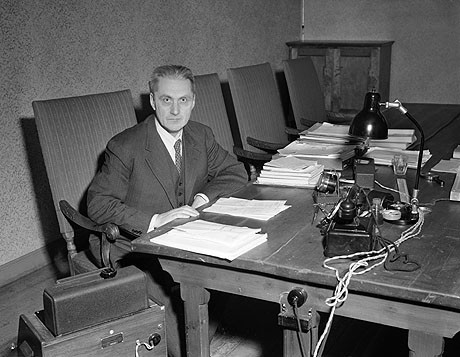
\includegraphics[width=.8\columnwidth]{frisch0}
\end{figure}
\end{frame} 

\begin{frame}{Ragnar Frisch}
\begin{figure}[H]
\centering

\includegraphics[width=.85\columnwidth]{frisch1}
\end{figure}
\end{frame} 

\begin{frame}{A Classic Example: Keynes' Consumption Function}
	\begin{itemize}
		\item Keynes' (1936) in his General Theory of Employment, Interest, and Money proposed the ``consumption function''
		\bigskip
		\item  This models the propensity to consume is a relationship $f$ between income $I$ and consumption $C$. 
		\bigskip
		\item His theory postulates that 
			\begin{enumerate}
				\item As a rule and on average, consumption increases as income increases but not as much as the increase in consumption
				\item As a rule, a greater proportion of income is saved as real consumption increases
			\end{enumerate}
	\end{itemize}
\end{frame}
 
\begin{frame}{Interpreting Keynes' Consumption Function}
	\begin{itemize}
		\item The function: $C = f (I)$
		\bigskip
		\item The marginal propensity to consume (MPC), defined as $\frac{dC}{dI}$, is such that $0 < \frac{dC}{dI} < 1$
		\bigskip
		\item The average propensity to consume (APC), defined as $\frac{C}{I}$, falls as income increases: $\frac{d \frac{C}{I} }{d I}$
		\bigskip
		\item Econometrics enables testing this theory
	\end{itemize}
\end{frame}

\begin{frame}{Testing Keynes' Theory}
	\begin{itemize}
	\item Postulate a linear relationship between $C$ and $I$: 
	\begin{align} 
	C = \alpha + \beta \cdot I \nonumber
	\end{align}
		\begin{itemize}
			\item $\alpha$: base consumption (independent of income level)
			\item $\beta$: MPC
		\end{itemize}
	\bigskip
	\item The first postulate is that $0 < \beta < 1$
	\bigskip
	\item The second postulate is that, if it could be recovered for groups with different income, $\beta$ would decrease as the level of income increases
	\end{itemize}
\end{frame}

\begin{frame}{A Fundamental Relationship in the Economics of Education}
\begin{itemize}
\item The relationship between the wage and years of schooling
\begin{align}
\log (\text{wage}) = \alpha + \beta \cdot \text{years of education} \nonumber
\end{align}
		\begin{itemize}
			\item $\alpha$: base wage level
			\item $\beta$: ``return to education'' 
		\end{itemize}
\end{itemize}
\end{frame} 

\begin{frame}{Examples of Other Fundamental Relationships in Economics}
	\begin{enumerate}
		\item Economic growth and monetary policy
		\bigskip
		\item Labor force participation and taxes
		\bigskip
		\item Lifetime income and elite college attendance 
		\bigskip
		\item Student performance and class size
		\bigskip
		\item Medical check-ups and health insurance
	\end{enumerate}
\end{frame}


\begin{frame}[noframenumbering]{Linear Regression: Learning the Relationship from the Data}
	\begin{itemize}
		\item The researcher postulates an economic model
			\begin{align}
				y = \alpha + x \cdot \beta \nonumber
			\end{align}
		\item And an empirical model
			\begin{align}
				y = \alpha + x \cdot \beta + \varepsilon, \nonumber
			\end{align}
		\noindent in which $\varepsilon$ enables modeling the ``unobserved difference'' between the model and the data
		\bigskip
		\item $\alpha$, $\beta$: parameters
		\item $y$, $x$, $\varepsilon$: random variables
		\bigskip
		\item A common, strong assumption: $\mathbb{E} \left[\varepsilon | x \right] = 0$
	\end{itemize}
\end{frame} 

\begin{frame}[noframenumbering]{Wage and Years of Education: A Linear Model}
\begin{figure}[H]
\centering
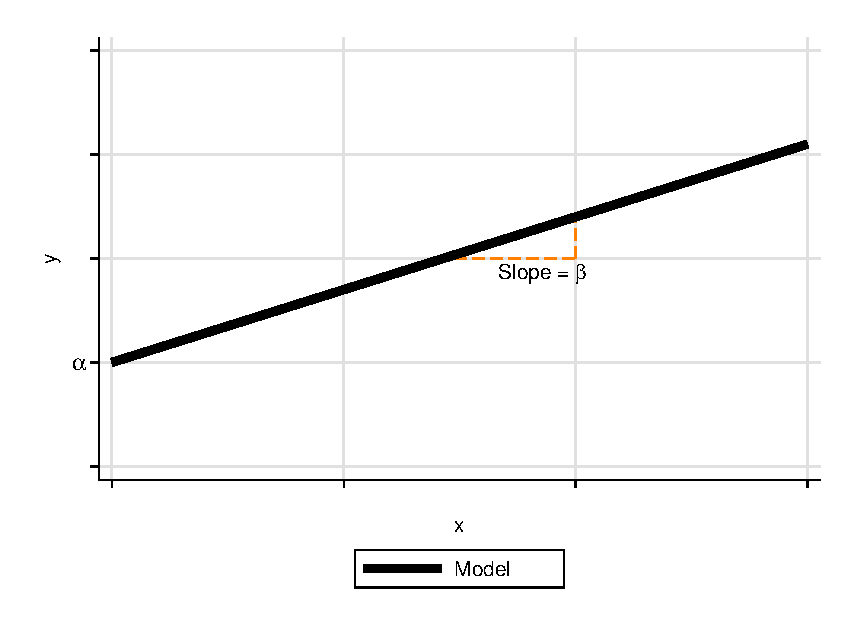
\includegraphics[width=.85\columnwidth]{linear_math}
\end{figure}
\end{frame} 

\begin{frame}[noframenumbering]{Wage and Years of Education: A Linear Model and the Population Data}
\begin{figure}[H]
\centering
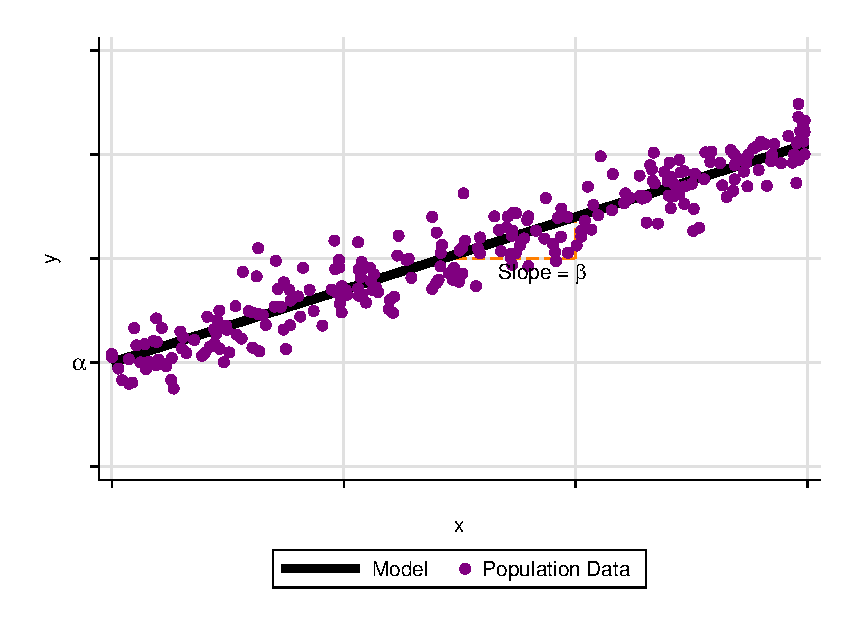
\includegraphics[width=.85\columnwidth]{linear_empirical}
\end{figure}
\end{frame} 

\begin{frame}{The Empirical Model in the Sample}
	\begin{itemize}
		\item The economic model aims to describe a population
		\bigskip
		\item Empirical analysis is performed on a sample
		\item A way to denote the distinction is
			\begin{align}
				y = a + x \cdot b + e, \nonumber
			\end{align}
	\noindent the parameters $\alpha$ and $\beta$ and the variable $\varepsilon$ are relabeled to distinguish between the population and the sample
	\bigskip
		\item $a$, $b$: parameters
		\item $y$, $x$, $e$: random variables
	\end{itemize}
\end{frame}

\begin{frame}{Population and Sample Regression: Terminology}
	\begin{itemize}
		\item Empirical model: $y = \alpha + x \cdot \beta + \varepsilon$
		\bigskip
		\item Population regression: $\mathbb{E} \left[ y | x \right]  = \alpha + x \cdot \beta$
		\item Sample regression (prediction): $\hat{y} := a + x \cdot b$
		\bigskip
		\item Error: $\varepsilon:= y - \alpha + x \cdot \beta$
		\item Residual: $e:= y - a + x \cdot b$
	\end{itemize}
\end{frame}

\begin{frame}{Population and Sample Regression: Visual Representation}
\begin{figure}[H]
\centering
\includegraphics[width=.85\columnwidth]{popsamplereg}
\end{figure}
\end{frame}

\begin{frame}{Econometric Tasks}
	\begin{enumerate}
		\item Postulate a model 
		\bigskip
		\item Obtain a sample that represents the population of interest
		\bigskip
		\item Estimate $a$ and $b$
		\bigskip
		\item Make inferences about $\alpha$ and $\beta$
		\bigskip 
		\item Conclude about the empirical content of the economic model
	\end{enumerate}
\end{frame}

\begin{frame}{Why is Inference about $\beta$ Important?}
	\begin{itemize}
		\item By definition, $\beta$ is the change in $\mathbb{E}\left[ y | x \right]$ given a one-unit increase in $x$
		\bigskip
		\item Inference about $\beta$ enables answering policy questions
		\item Example: Is it the case that $0 < \text{MPC} < 1$? 
		\bigskip
		\item The model holds as long as $\mathbb{E}\left[\varepsilon | x \right] = 0$
		\item That is, the relationship is causal under such assumption
	\end{itemize}
\end{frame}


\begin{frame}{$\mathbb{E} \left[ \varepsilon | x \right] = 0$: Visual Representation}
\begin{figure}[H]
\centering
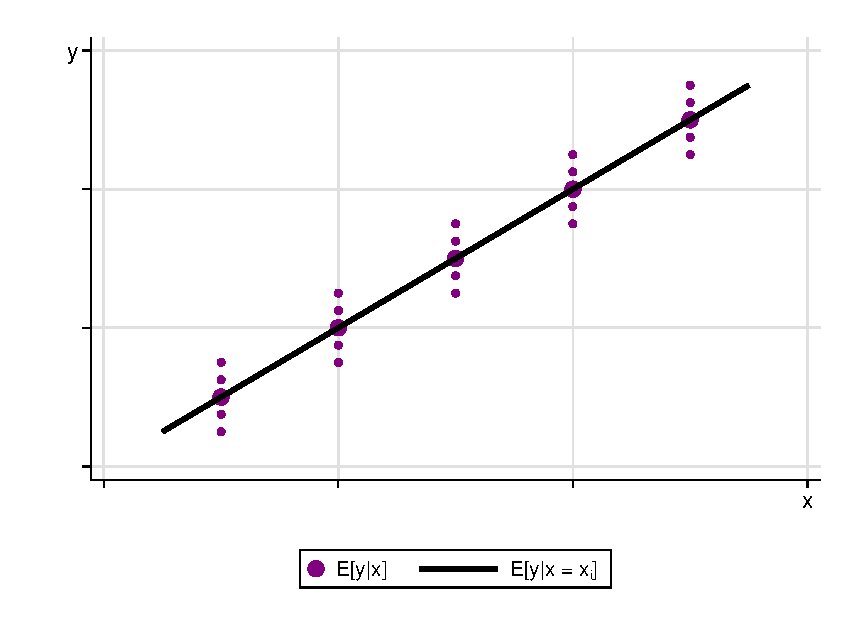
\includegraphics[width=.85\columnwidth]{conditionalexpected}
\end{figure}
\end{frame}

\begin{frame}{A Practical Way of Thinking About $\mathbb{E} \left[ \varepsilon | x \right] = 0$}
		\begin{itemize}
			\item Note that $\mathbb{E} \left[ \varepsilon | x \right] = 0$ implies that $\mathbb{E} \left[ \varepsilon \right] = 0$. 
			\item  $\mathbb{E} \left[ \varepsilon | x \right] = \mathbb{E} \left[ \varepsilon \right]$  implies that $\cov \left( x, \varepsilon \right) = 0$ 
			\bigskip
			\item Arguments in favor of (or against) $\mathbb{E} \left[ \varepsilon | x \right] = 0$ are usually arguments in favor of (or against) $\cov \left( x, \varepsilon \right) = 0$
		\end{itemize}
\end{frame}

\begin{frame}{Correlation is No Causation}
		\begin{itemize}
			\item Consider the model 
			\begin{align}
			\log (\text{wage}) = \alpha + \beta \cdot \text{years of education} + \varepsilon \nonumber
			\end{align}
		\item Is it true that $\cov \left( \text{years of education}, \varepsilon \right) = 0$? 
		\item $\cov \left( \text{years of education}, \varepsilon \right) > 0$ could generate an ``spurious correlation'' between the wage and years of education
		\bigskip
		\item Generally, people with more years education have higher wages (positive correlation). That does not mean that the years of education \textit{cause} higher wages 
		\end{itemize}	
\end{frame}

\begin{frame}{Economic and Statistical Exercises}
	\begin{itemize}
	\item Justifying $\cov \left( x, \varepsilon \right) = 0$ is an economic exercise
		\begin{itemize}
			\item Justifaibility depends on the model and the context
			\item Unverifiable by construction: It is an assumption about the unobserved term $\varepsilon$
		\end{itemize}
	\bigskip
	\item Estimation and inference are statistical exercises 
		\begin{itemize}
			\item Estimate $a$ and $b$ to make inference about $\alpha$ and $\beta$ 	
			\item They are possible even if $\mathbb{E} \left[ \varepsilon | x \right], \cov \left( x, \varepsilon \right) \neq 0$
		\end{itemize}
	\end{itemize}
\end{frame}

\begin{frame}{Estimation: Ordinary Least Squares}
	\begin{itemize}
	\item With a sample in hand, the aim is to estimate the coefficients in 
		\begin{align}
			y = a + x \cdot b + e  \nonumber
		\end{align}
	\item Idea: To ``choose'' the coefficients $a$ and $b$ that best ``fit'' the sample 
	\item Execution: Minimize the quadratic sum of squares in the sample
	\end{itemize}
\end{frame}

\begin{frame}{OLS: Visual Representation}
	\begin{figure}[H]
	\centering
	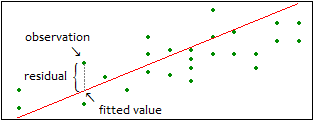
\includegraphics[width=.85\columnwidth]{fitted}
	\end{figure}
	\begin{itemize}
	\item The estimated fitted value for each value of $x$ is $\hat{a} + x \cdot \hat{b}$, where $\hat{a}$ and $\hat{b}$ are estimates of $a$ and $b$
	\item The estimated residual for each value of $x$ is $\hat{e}:= y - \hat{a} - x \cdot \hat{b}$
	\end{itemize}
\end{frame}

\begin{equation}



%%--------------------------- Content ends here ---------------------------------------------------
%%

% --------------------- Bibliography hidden with a save box ---------------------------------------
\mode<all>
\bibliographystyle{chicago}
\savebox\hiddenbib{\parbox{\textwidth}{\bibliography{hocp_jlg}}}

\end{document} 
